\documentclass[12pt,a4paper]{article} 

\title{NeuroField Reference}
\author{Peter Drysdale \and Felix Fung \and Romesh Abeysuriya}
\date{\today}

\usepackage[latin1]{inputenc}
\usepackage{tikz}
\usetikzlibrary{shapes,arrows}

\usepackage{listings}
\usepackage{hyperref}
\usepackage{graphicx}
\usepackage[top=2cm,bottom=2cm,left=1.3cm,right=1.3cm]{geometry}
\usepackage{multirow}
\usepackage{amsmath}

\pagestyle{plain}
\parindent=0.0cm
\parskip=0.5cm

\footskip=1.3cm

\lstset{
basicstyle=\small\small\ttfamily,
frame=single,	        % adds a frame around the code
breaklines=true,		% sets automatic line breaking
breakatwhitespace=tru,	% sets if automatic breaks should only happen at whitespace
}
\newcommand{\code}[1]{ 
\begin{lstlisting}
#1
\end{lstlisting}
}
\newcommand{\type}[1]{ {\small\small\tt #1} }

\newcommand{\NF}[0]{ \type{NeuroField}}

\begin{document}

\maketitle
\abstract{\NF is a computer program (accompanied with helper scripts) that solves the neural field model of Robinson et al. This document is a reference of \NF for both users and developers.}
\tableofcontents

\pagebreak
\section{Users guide}

\NF, written by Peter Drysdale with contributions from James Roberts, Felix Fung and Romesh Abeysuriya, is a \type{C++} program (accompanied with helper scripts) that solves the neural field model of Robinson et al.:
\begin{align*}
	D_{ab}V_{ab}(\mathbf{r},t) &= \nu_{ab}\phi_{ab}(\mathbf{r},t),\\
			Q_a(\mathbf{r},t) &= S_a \big[\sum_b V_{ab}(\mathbf{r},t) \big],\\
	\mathcal{D}_{ab}\phi_{ab}(\mathbf{r},t) &= Q_b(\mathbf{r},t-\tau_{ab}).
\end{align*}
\NF generalizes the neural field theory by allowing users to:
\begin{enumerate}
	\item Specify an arbitrary number of populations and connections between populations;
	\item Specify the parameters for any objects, including populations, dendritic responses, firing responses, propagators, synapses, and stimulus pattern;
	\item Choose alternative wave propagation types, i.e. choose different forms of \(\mathcal{D}_{ab}\);
	\item Uses plastic synapses, i.e. \(\nu_{ab}=\nu_{ab}(\mathbf{r},t)\).
	\item Use different firing responses, i.e. change \(S_a\).
\end{enumerate}

This users guide covers the obtaining and setting up (Sec.~\ref{sec:obtain}), configuring (Sec.~\ref{sec:config}) and launching of \NF (Sec.~\ref{sec:launch}).

Within this documentation, specific terminology as appeared in the computer is in \type{typwriter font}. Commands are denoted as
\begin{lstlisting}
Command to put in computer
\end{lstlisting}

\subsection{Obtaining and setting up \NF}
\label{sec:obtain}

The code for \NF is managed by a version control system called \type{subversion}, which provides a single place to obtain the latest copy of the code, as well as storing the entire history of the program. To access the repository, contact Romesh Abeysuriya (\url{r.abeysuriya@physics.usyd.edu.au}) or Sue Yang (\url{xue.yang@sydney.edu.au}).

To set up the latest version of \NF in the current directory within the School of Physics, execute
\begin{lstlisting}
svn co http://silliac.physics.usyd.edu.au:18080/svn/neurofield/trunk neurofield --username=<your SVN username>
\end{lstlisting}

You can also use these steps to obtain a copy of \NF from a computer which is not connected to the School of Physics network (eg. personal laptops at home). You will require a version of \type{SVN} higher than 1.6. However, you may need to have your IP address/network domain registered for remote access. If you are unable to access the repository remotely, please contact Sebastian Juraszek to request this (ideally by logging a helpdesk request at \url{http://physics.usyd.edu.au/itsupport} - only available within the School of Physics). 

\subsection{Directory layout}

The canonical directory is \type{neurofield/trunk}. Within this directory, the user can find:

\begin{tabular}{l p{12cm}}
\type{*.h, *.cpp}& C++ source code.\\
\type{Configs/}& Stores configuration files for \NF.\\
\type{Documentation/}& \type{Documentation/doc.tex} is the \LaTeX\ file for generating this document. Running \type{make doc} produces this document in \type{pdf} format, and \type{make clean} removes all the files \LaTeX\ produced (excluding \type{doc.pdf} and \type{doc.tex}).\\
\type{Helper\_scripts/}& Stores helper scripts, including plotting routines and other post-processing of data procedures.\\
\type{Launch}& A launcher script that handles compilation and launching of \NF, capable of automating parameter sweeps and submitting jobs in \type{yossarian}.\\
\type{Output/}& When using the launcher script to sweep over parameters, the launcher script produces this directory, which stores all output files \type{neurofield.*} in independent subdirectories.\\
\type{Release/}& All compiled files, including the object files and the \NF executable is stored here. This directory will be deleted by \type{make clean}, so user data should not be stored here.\\
\type{Test/}& Directory for unit testing and is irrelevant for users.\\
\type{neurofield.*}& Output files generated by \NF.
\end{tabular}

\subsection{Launching NeuroField}
\label{sec:launch}

The \type{Launch} script is used to compile and launch the \NF program. Users are encouraged to use this script rather than calling the \NF executable directly. To launch \NF, do:

\begin{enumerate}

\item Edit \type{Makefile}: Identify the platform to run NeuroField, and comment/uncomment the appropriate \type{COMP} directions. Generally, this step is not needed, but users are encouraged to check.

\item To execute with only one set of parameters, edit your configuration file in \type{./Configs}, then run
\begin{lstlisting}
./Launch Configs/config_file
\end{lstlisting}
For example,
\begin{lstlisting}
./Launch Configs/cortex.conf
\end{lstlisting}
The output will be stored in the current directory.\footnote{Tips for \type{vi} users: you can launch \NF in \type{vi} with \type{:!./Launch \% [optional params]} }

\item To ease parameter exploration, the launcher script is capable of doing parameter sweeps. The launcher script supports sweeping over an arbitrary number of objects, parameters and runs. For example, if the user wants to launch \NF 3 times, with parameters varying according to the following table,

\begin{tabular}{l l r r r}
Object(s)&Parameter&1\textsuperscript{st} run&2\textsuperscript{nd} run&3\textsuperscript{rd} run\\
\hline
\type{Propag 1}, \type{Propag 2}&\type{gamma}&10&20&30\\
\type{Couple 1}&\type{nu}&1&2&3
\end{tabular}

simply list the above table entries into the argument list:
\begin{lstlisting}
./Launch Configs/cortex.conf 'Propag 1' 'Propag 2' gamma 10 20 30 'Couple 1' nu 1 2 3
\end{lstlisting}

In terms of syntactic restriction, each row in the table can have an arbitary number of objects, but only one parameter; every row must have the same number of runs.\footnote{Tips: the UNIX \type{seq} program allows shortening parameter value listing from \type{10 20 30 40 50 60} into \type{`seq 10 10 60`}, e.g. \type{Launch Configs/cortex.conf 'Propag 1' gamma `seq 10 10 60`}.}

\item Switches are accepted for choosing options. To turn on the switches, put them in the argument list to the launcher script. The following switches are accepted:
	\begin{description}
	\item[\type{--restart}] run \NF in restart mode.
	\item[\type{-i}] specify an configuration file name.
	\item[\type{-o}] specify an output dump file name.
	\item[\type{-v}] prints to standard output rather than to a file.
	\item[\type{-h}] prints out a list of these switches.
	\end{description}

\item In case the script is executed on \type{yossarian}, the launcher script tries to find a file called \type{pbs}. If no such file is found, the user would be prompted for a job name, expected computational time and email to generate \type{pbs}. This file is then submitted to the PBS system.

\item To clean up the directory, delete or store your \type{neurofield.*} output files and the \type{Output/} directory and subdirectories. Then run
\begin{lstlisting}
make clean
\end{lstlisting}
to delete \type{./Release/} and the files \LaTeX produced in \type{Documentation/}.

\item This documentation can be generated by running 
\begin{lstlisting}
make doc
\end{lstlisting}
which produces \type{./Document\-ation.pdf}. \type{make clean} deletes the files (excluding \type{./Document\-ation.pdf}) created by \LaTeX.

\end{enumerate}

%\subsection{Using NeuroField executable without launcher script}
%\label{sec:exe}

%It is possible to use the launcher script in virtually all cases, so that a user may skip this section. A notable exception is to restart a completed simulation with a \type{neurofield.dump} file. If a user wishes to use the \type{./Release/NeuroField} executable without the launcher script, then compile it by running
%\begin{lstlisting}
%make
%\end{lstlisting}
%The \NF executable and object files are produced in \type{./Release/}.

%The \type{./Release/NeuroField} executable runs in one of two modes, initial run mode and restart mode.

%(1) In inital run mode \NF takes input from an \type{neurofield.conf} file initializes the simulation and then takes specified number of integration steps writing out a \type{neurofield.output} file and a \type{neurofield.dump} file for restarting.  The input filename can be changed on the command line by using the switch \type{-i newinputfilename}. Similarly the name of the output filename which defaults to \type{neurofield.output} can be changed via the switch \type{-o newoutputfilename}. The dump file which defaults to \type{neurofiled.dump} can be changed via \type{-d newdumpfilename}.

%(2) The code dumps sufficient data about parameter values to restart. In restart mode the simulation will continue where it left off. Restart mode is accessed by running the code with command \type{Neurofield restart} rather than the usual \NF command on the command line. In order to run the code in restart mode it is necessary to take the \type{neurofield.dump} file which was produced from the run which will be restarted to be renamed as the new \type{neurofield.conf} file. The new \type{neurofield.conf} file should also be changed to reflect the new number of timesteps etc.  Note:- A restarting \type{neurofield.conf} file has different content to an initial run \type{neurofield.conf} and can only be used in restart mode.

%A brief description is given by
%\begin{lstlisting}
%./Release/NeuroField --help
%\end{lstlisting}

\subsection{Writing a configuration file}
\label{sec:config}

\NF allows an arbitrary number of populations and connections between them, with all objects taking arbitrary parameter values. These are all configured via a configuration file. This section documents the specifications of configuration files, where we use \type{Configs/cortex.conf} as an illustrative example.

To write a configuration file, a user can follow these steps:
\begin{enumerate}
\item Determine your population model by drawing a schematic diagram, thereby constructing a connection matrix. An example is shown in Fig.~\ref{fig:pop}.
\item Look up existing configuration files in \type{Configs/}. By checking the comment located at the top of a configuration file, and also the connection matrix, a user should find the most suitable existing file to construct his own. This is less tedious (and less error prone) than writing a new one from scratch.
\item Specify the global parameters and connectivity matrix (Sec.~\ref{sec:global}).
\item Specify all populations (Sec.~\ref{sec:pop}).
\item Specify all propagators (Sec.~\ref{sec:prop}).
\item Specify all couples (Sec.~\ref{sec:couple}).
\item Specify all output requests (Sec.~\ref{sec:output}).
\end{enumerate}

\begin{figure}[h!]\begin{center}
\tikzstyle{block} = [draw,text width=3em,text centered,minimum height=2em]
\tikzstyle{line} = [draw, -latex']
    
\begin{tikzpicture}[node distance = 3em, auto]
	\node[block] (epsilon) {$\epsilon$};
	\node[right of=epsilon,node distance=4em](epsilone){};
	\path[line](epsilon)--(epsilone);
	\node[block, right of=epsilone] (e) {e};
	\path[line] (epsilon) -- (e);

	\node[right of=e](re){};
	\draw(e)--(re);
	\node[above of=re](are){};
	\draw(re)--(are);
	\node[left of=are](ae){};
	\draw(are)--(ae);
	\path[line] (ae) -| (e);

	\node[block, below of=epsilon] (iota) {$\iota$};
	\node[right of=iota,node distance=4em](iotai){};
	\path[line](iota)--(iotai);
	\node[block, right of=iotai] (i) {i};
	\path[line] (iota) -- (i);

	\node[right of=i](ri){};
	\draw(i)--(ri);
	\node[below of=ri](bri){};
	\draw(ri)--(bri);
	\node[left of=bri](bi){};
	\draw(bri)--(bi);
	\path[line] (bi) -| (i);

	\path[line] (e) -- (i);
	\path[line] (iotai) -- (epsilone);
\end{tikzpicture}
\hspace{3cm}\begin{tabular}{ l l l l l }
	From:& $\epsilon$ & $\iota$ & e & i \\
	To $\epsilon$:& 0 & 0 & 0 & 0 \\
	To $\iota$:& 0 & 0 & 0 & 0 \\
	To e:& 1 & 0 & 2 & 3 \\
	To i:& 0 & 4 & 5 & 6
\end{tabular}
\caption{Left: schematic diagram of a purely cortical population model comprising excitatory and inhibitory populations, as well as two stimulus populations; each arrow indicates a connection between populations, so that each stimulus connects to a cortical population, and each cortical population connects to all cortical populations. Right: connection matrix indicating the connections between populations; zero indicates no connection, and a connection is indicated by a nonzero number, ordered top to bottom, left to right.}
\label{fig:pop}\end{center}\end{figure}


\begin{figure}\begin{center}
	\begin{lstlisting}
Purely cortical model with excitatory and inhibitory neurons
Time: 10 Deltat: 1e-4
Nodes: 4

Connection matrix:
From: 1 2 3 4
To 1: 0 0 0 0
To 2: 0 0 0 0
To 3: 1 0 2 3
To 4: 0 4 5 6

Population 1: Stimulation
 Stimulus: Const - Onset: 0 Mean: 5

Population 2: Stimulation
 Stimulus: Const - Onset: 0 Mean: 5

Population 3: Excitatory neurons
 Q: 8.87145
 Firing: Sigmoid - Theta: 13e-3 Sigma: 3.8e-3 Qmax: 340
  Dendrite 1: V: Steady alpha: 83 beta: 769
  Dendrite 2: alpha: 83 beta: 769
  Dendrite 3: alpha: 83 beta: 769

Population 4: Inhibitory neurons
 Q: 8.87145
 Firing: Sigmoid - Theta: 13e-3 Sigma: 3.8e-3 Qmax: 340
  Dendrite 4: V: Steady alpha: 83 beta: 769
  Dendrite 5: alpha: 83 beta: 769
  Dendrite 6: alpha: 83 beta: 769

Propag 1: Map  - Tau: 0
Propag 2: Wave - Tau: 0 Deltax: 3.5e-3 Range: 80e-3 gamma: 116
Propag 3: Map  - Tau: 0
Propag 4: Map  - Tau: 0
Propag 5: Wave - Tau: 0 Deltax: 3.5e-3 Range: 80e-3 gamma: 116
Propag 6: Map  - Tau: 0

Couple 1: Map - nu: .15e-3
Couple 2: Map - nu: 1.5e-3
Couple 3: Map - nu:-1.8e-3
Couple 4: Map - nu: .15e-3
Couple 5: Map - nu: 1.5e-3
Couple 6: Map - nu:-1.8e-3

Output: Node: All
Population: 
Dendrite:
Propag: 3 4
Couple:
	\end{lstlisting}
\end{center}
\caption{An example configuration file, which can be found in \type{Configs/cortex.conf}.}
\end{figure}

In general, the entries in configuration file follow the following rules:

\begin{enumerate}
	\item Each entry generally follows a \type{Pamameter: value} pattern.
	\item Most parameters are essential. Failure to provide these parameters would result in \NF terminating with an error message. A minority of the parameters are optional.
	\item The ordering of the parameters are important. Wrong parameter ordering results in \NF terminating with an error message.
	\item With the exception of keywords, the configuration file is white-space independent, e.g., there can be either no spaces, many spaces, or new lines between the colon of \type{Integration steps: 10000} and 10000, but you cannot have two spaces between \type{Integration} and \type{steps}. For consistency and readability, users are encouraged to follow the existing white space scheme when reasonable.
	\item Tip for \type{vi} users: \type{./helper\_scripts/neurofield.vim} implements syntax highlighting for configuration files in \type{vi}. See comments within for installation instructions.
\end{enumerate}

\subsubsection{Global information}
\label{sec:global}
\begin{itemize}

\item
\begin{lstlisting}
Purely cortical model with excitatory and inhibitory neurons
\end{lstlisting}
Any text before the entry, \type{Time:}, is disregarded by \NF and serves as comment.
\item
\begin{lstlisting}
Time: 10 Deltat: 1e-4
\end{lstlisting}
\type{Time} is the simulation duration in seconds.

\type{Deltat} is the time increment for each time step.
\item
\begin{lstlisting}
Nodes: 4 Longside: 2
\end{lstlisting}
\type{Nodes} is the number of grid points in the spatial dimension per population of neurons. The code has been explicitly designed to have equal number of neurons per population.

\type{Longside} is an optional parameter, specifying the longside of the rectangular grid. If it is not supplied, it is assumed to be a square.

Both spatial dimensions have periodic boundary conditions, so that populations have the topology of a torus.
\item
\begin{lstlisting}
Glutamate dynamics - fast Lambda: 3e-4 fast tGlu: 5e-3
                     slow Lambda: 3e-4 slow tGlu: 5e-3
\end{lstlisting}
Parameters governing glutamate dynamics, which is currently useful only for \type{CaDP}. This block is optional.

\type{Lambda} is the glutamate release concentration per presynaptic spike, in moles.

\type{tGlu} is the decay timescale of glutamate in seconds.
\item
\begin{lstlisting}
Connection matrix:
From: 1 2 3 4
To 1: 0 0 0 0
To 2: 0 0 0 0
To 3: 1 0 2 3
To 4: 0 4 5 6
\end{lstlisting}
We specify an arbitrarily sized square connection matrix, where each entry is the connection from the column population to the row population.

Zero indicates no connection.

A nonzero number indicates connection. This number must be indexed from top to bottom, left to right.
\end{itemize}

\subsubsection{Population data}
\label{sec:pop}
This section contains population information sections. There are two types of neural populations: ordinary populations and stimulus populations:
\begin{description}

\item[Stimulus populations]\ \\

\NF identifies stimulus populations as populations which have no dendrites, i.e., the row for that population contains no nonzero elements.  Each stimulus population information section is as follows.
\begin{itemize}
	\item \begin{lstlisting}
Population 1: Stimulation
	\end{lstlisting}
	The identifier \type{Population 1} is required for cross-checking.

	The descriptor \type{Stimulation} is not parsed by \NF, but it is strongly recommended for human referencing.
	\item
	\begin{lstlisting}
Stimulus: Const - Onset: 0
	\end{lstlisting}
	The identifier \type{Stimulus} is required for cross-checking.

	This is followed by the type of stimulus, to be further elaborated below.

	Optional parameter \type{Onset} specifies the time onset for the stimulus to begin. If unspecified, stimulus starts at time 0.

	Either \type{Cease} or \type{Duration} can be an optional parameter to specify the end time of the stimulus. If unspecified, stimulus ends at 1000 seconds.

	Possible stimulus patterns:

	\textbf{Constant}
	\begin{lstlisting}
Const - Mean: 5
	\end{lstlisting}

	\textbf{Pulse}
	\begin{lstlisting}
Pulse - Amplitude: 1 Width: 2e-2 Frequency: 1 Pulses: 1
	\end{lstlisting}

	\textbf{White noise stimulus}
	\begin{lstlisting}
White - Amplitude: 20 Mean: 1
	\end{lstlisting}

    One issue with white noise is that the power spectrum of white noise depends on both the temporal sampling rate and the grid size. For a thorough discussion of this phenomenon, see \type{noise.pdf} in the \NF documentation. Therefore, if you change the sampling rate, the number of nodes, or \type{Deltax} then the power spectrum will change in amplitude. If you know what amplitude the noise should have in Fourier space e.g. $\phi_n(\omega) = 1 \times 10^{-5}$ then specifying \type{Deltax} in the stimulus population will tell \NF that the amplitude has been specified in Fourier space, and it will be rescaled accordingly. In this representation, the mean of the distribution corresponds to the zero-frequency component of the noise. 
    
	\begin{lstlisting}
White - Amplitude: 0.00001 Mean: 1 Deltax: 0.025
	\end{lstlisting}
	
	Whether \type{Deltax} is specified or not, you can always optionally specify the seed for the random number generator. If you do not specify a seed, an automatically-incremented seed will be used instead, so that multiple stimulus populations will have independent sequences. In general it is not necessary to set the seed manually unless different random numbers are required for otherwise identical runs. 

	\begin{lstlisting}
White - Amplitude: 0.00001 Mean: 1 Ranseed: 10
	\end{lstlisting}
	\begin{lstlisting}
White - Amplitude: 0.00001 Mean: 1 Deltax: 0.025 Ranseed: 10
	\end{lstlisting}

	To superimpose 2 or more stimuli, begin with the keyword \type{Superimpose}, followed by the number of stimuli. Then list all the stimulus patterns and their parameters, with each stimulus pattern preceded by the keyword \type{Stimulus}.
	\begin{lstlisting}
Stimulus: Superimpose: 2
 Stimulus: White - Amplitude: 1 Mean: 1
 Stimulus: Pulse - Onset: 0.5 Width: 2e-2 Frequency 1 Pulses: 1
	\end{lstlisting}

	\end{itemize}
\item[Ordinary populations]\ \\
	Any non-stimulus population is an ordinary population.

	\begin{itemize}
	\item
	\begin{lstlisting}
Population 3: Excitory neurons
	\end{lstlisting}
	The identifier \type{Population 3} is required for cross-checking.
	
	The descriptor \type{Excitatory neurons} is not parsed by \NF, but it is strongly recommended for human referencing.
	\item
	\begin{lstlisting}
Q: 8.87145
	\end{lstlisting}
	The initial firing rate.
	\item
	\begin{lstlisting}
Firing: Sigmoid - Theta: 13e-3 Sigma: 3.8e-3 Qmax: 340
	\end{lstlisting}
	Specify the sigmoidal firing response of the population.

	\type{Sigma} is sometimes known as \(\tilde{\sigma}\). It is already scaled by \(\pi/\sqrt{3}\).

	Alternatively, you can specify a linear firing response by using
	\begin{lstlisting}
Firing: Linear - Gradient: 1 Intercept: 1
	\end{lstlisting}

	\item
	\begin{lstlisting}
Dendrite 1: V: Steady alpha: 83 beta: 769
	\end{lstlisting}
	The identifier \type{Dendrite 1}, where 1 is the presynaptic connection index, is required for cross-checking. Users should find that these indices are simply ordered as 1, 2, 3, 4, ...
	
	\type{V} is the initial depolarization contribution from presynaptic activity. It can be a numerical value with units of V, or set at \type{Steady}, so that \NF calculates the initial value by \(V_{ab}=\nu_{ab}\phi_{ab}\).

	\type{alpha} and \type{beta} are the parameters for the depolarization response.
	\end{itemize}
\end{description}

\subsubsection{Propagation data}
\label{sec:prop}
\item
	\begin{lstlisting}
Propag 1:
	\end{lstlisting}
	This identifier is required for cross-checking.
\item A propagator type is required at this point. Choices are \type{Map}, \type{Wave}, and \type{Harmonic}.
\begin{description}
	\item[Map]\ \\
	\begin{lstlisting}
Map - Tau: 0
	\end{lstlisting}
	This propagator is the mapping propagator where spatial spreading is negligible. Its form is given by
	\[\phi_{ab}({\bf r}, t) = Q_b ({\bf r}, t - \tau_{ab}).\]
	Its only one parameter, \type{Tau}, is the the delay term. It is specified below.

	\item[Wave]\ \\
	This propagator is the wave equation propagator governed by the equation
	\[\left[\frac{1}{\gamma_{ab}^2}\frac{d^2}{d t^2}+\frac{2}{\gamma_{ab}}\frac{d} {d t}+1 \right] \phi_{ab}({\bf r},t) =Q_b({\bf r},t-\tau_{ab}).\]
	Its input is given by
	\begin{lstlisting}
Wave - phi: Steady Deltax: 0.0035 Tau: 0 Range: 0.08 gamma: 116
	\end{lstlisting}
	\type{phi} is the initial value for $\phi_{ab}$ in the wave equation. Inputting \type{Steady} gives \(\phi_{ab} = Q_b\).

	\type{Deltax} is the length of a node in mm. This must satisfy the Courant condition, \[\Delta t/\Delta x<\sqrt{2}/r_e\gamma_e.\]

	\type{Range} is $r_{ab}$ in the wave equation.
	
	The final parameter can be \type{gamma} or \type{velocity} in the wave equation.

	In case there is only one node, this degenerates into a \type{Harmonic} propagator.

	\item[Harmonic]
	This is a harmonic oscillator implementation of the damped wave equation. If there is no spatial variation, use \type{Harmonic} instead of \type{WaveEqn}.
	The input form is given by 
	\begin{lstlisting}
Harmonic - phi: Steady Tau: 0 gamma: 116
	\end{lstlisting}

	\item[Tau]\ \\
	The axonal time delay between populations. If it is spatially homogeneous, then it is a number with units of seconds. If it is spatially inhomogeneous, then input \(n\) numbers, where \(n=\) \type{Nodes}.

\end{description}

\subsubsection{Coupling data}
\label{sec:couple}

\begin{itemize}

	\item
	\begin{lstlisting}
Couple 1:
	\end{lstlisting}
	Identifier for cross-checking.
\item A couple type is required at this point. Choices are \type{Map}, \type{CaDP}, \type{BCM} and \type{Matrix}.

\begin{description}

	\item[Map]\ \\
	Nonplastic synaptic coupling wtih a single constant parameter \type{nu},
	\begin{lstlisting}
Map - nu: 0.0012
	\end{lstlisting}
	\type{nu} is the synaptic coupling parameter. It corresponds to the product of the mean synaptic strength $s_{ab}$ and $N_{ab}$, the mean number of connections from cells of type $b$ to cells of type $a$.

	%\item[Modcouple]\ \\
	%The modulated synaptic coupling implements the Clearwater/Rennie modulation equation. The modulation is given by
	%\[ \nu (t) = \nu_0 \left[ ( 1 - \nu_{scal} ) e^{h(t)/k} + \nu_{scal} \right], \]
	%where $h(t)$ is the time low passed filtered form of the neuromodulators concentration $C(t)$ as given by
	%\[
	%\left\{ \frac{1}{\mu \lambda} \frac{d^2}{dt^2} +
	%\left[ \frac{1}{\nu}+ \frac{1}{\lambda} 
	%\right]
	%\frac{d}{dt} + 1
	%\right\}
	%h(t) = C(t).
	%\]
	%The neuromodulator's concentration is in turn given by a user chosen stimulus form analogous to stimulus populations.

	%The remainder of the input form is specification of the output for $\nu$.  This takes an analogous form to the usual output data lines. The $\nu$ data is output to a file with filename \type{neurofield.synaptout.xx} where xx is an index number of the coupling.

	%An example Modcouple input form is given by
	%\begin{lstlisting}
%ModCouple - Nuzero: 0.0002 Nuscal: 0.02 Mu: .1 Lambda: 1 k: .000001
%Concentration mode: 1  Time to start of Concentration: .01 Amplitude: .0001
%Pulse Duration: .2 Pulse repetition period: 40
%Number of traces: 100  Single/All: All nodes}
	%\end{lstlisting}

	\item[Matrix]\ \\
	Coupling becomes connection matrix, where connection strength does \emph{not} change with time. The format of the nu matrix is the same as the population connection matrix, each row is to the same node, each column is from the same node. When outputting, each specified outputting node output the indexed row.
	\begin{lstlisting}
nu:
  13e-6 0
  0 13e-6
	\end{lstlisting}

	\item[CaDP]\ \\
	Calcium dependent plasticity according to Fung and Robinson.
	\begin{lstlisting}
CaDP - nu: 13e-6 nu_max: 80e-6 Dth: .25e-6 Pth: .45e-6 xyth: 1e-4 x: 2.3e-2 y: 2e-2 B: 30e3 glu_0: 200e-6 gNMDA: 2e-3
	\end{lstlisting}

	\item[BCM]\ \\
	BCM plasticity according to Fung and Robinson. Based on \type{CaDP}, it has an additional parameter \type{t\_BCM}.
	\begin{lstlisting}
CaDP - nu: 13e-6 nu_max: 80e-6 Dth: .25e-6 Pth: .45e-6 xyth: 1e-4 x: 2.3e-2 y: 2e-2 B: 30e3 glu_0: 200e-6 gNMDA: 2e-3 t_BCM: 7
	\end{lstlisting}

\end{description}
\end{itemize}

\subsubsection{Output data}
\label{sec:output}

\NF outputs field quantities (i.e. a neurodynamic quantity which takes a value for each node) with respect to nodes and time. By default, the output file is \type{neurofield.output}, which can be changed by launching the program with the \type{-o} switch.

\begin{itemize}
	\item \begin{lstlisting}
Output:
		\end{lstlisting}
Begin with the \type{Output} declaration.
\item \begin{lstlisting}
Node: 1 2
\end{lstlisting}
Enumerate all nodes to be outputted. If outputting all nodes, use shorthand \type{All}.
\item \begin{lstlisting}
Start: 0 Interval: 1e-3
\end{lstlisting}
Optional parameters for the time to start output, and optional parameter for time interval between outputs.

If undefined, defaults, to 0 and \type{Deltat}, respectively.
\item \begin{lstlisting}
Population: 2.V
Dendrite:
Propag: 1 2.phi
Couple: 3.nu
\end{lstlisting}
Specifying desired objects and fields to output. Enter the appropriate object indices after the labels. For each entry, a field name may be appended after the index with a \type{.}, so that only that field of the object is outputted. If no field name is specified for that entry, then all fields of that object is outputted.
\end{itemize}

\subsection{Postprocessing}

\NF produces 3 files:

\begin{tabular}{l p{11.5cm}}
\type{neurofield.conf}& When using the launcher script, this file is created to store the running configuration file.\\
%\type{neurofield.dump}& \NF dumps data here when it terminates. This file can be used in restart mode to continue simulation. Creation of this file can be suppressed by a \type{-s} switch.\\
\type{neurofield.output}& The result of the simulation is stored here for postprocessing.\\
\type{neurofield.pbs}& If \NF is run in \type{yossarian}, then this file stores the output of the queueing system.
\end{tabular}

When the launcher script runs with only one set of parameters, all output files are also in the present working directory. However, if the launcher script sweeps over parameters, each parameter set has its own subdirectory inside \type{Output/}, and each set of \type{neurofield.*} files are stored in its subdirectory.

Example content in \type{neurofield.output} is
\begin{lstlisting}
                Time  |          Propag.2.phi
                      |                     0
1.00000000000000e-04  |  8.87145000000000e+00
\end{lstlisting}

Each column is a time series with its name indicated in the first line. The first column is always time, and in this example, the second column is \type{Propag.2.phi}, indicating that it is $\phi_{ee}$ (when checked against connection matrix). The delimiter \type{|} indicates that the two columns are different fields, rather than different nodes of the same field. The node number is indicated in the second line.

It is also worth noting that traces will be written in the order that they are specified. For example, if you write \type{Population: 3 1} then the columns in the output file will be arranged in this order. 

\subsubsection{Quickplot}

The data in \type{neurofield.output} may be plotted by \type{./Helper\_script/quickplot.pl} or in \type{MatLab} via the matlab scripts within \type{./Helper\_script/}.

To use \type{./Helper\_script\/quickplot.pl}, execute
\begin{lstlisting}
./Helper_script/quickplot.pl [output.file] [field] [node index]
\end{lstlisting}
where an example is
\begin{lstlisting}
./Helper_script/quickplot.pl neurofield.output Propag.2.phi 1
\end{lstlisting}
or a shorthand to plot all fields and nodes is
\begin{lstlisting}
./Helper_script/quickplot.pl all
\end{lstlisting}
All these commands launches \type{gnuplot} plotting sessions.

\subsubsection{Matlab}
A number of Matlab functions are provided to make it easy to manipulate \NF data from within Matlab. The functions are generally self-documenting with comments at the start of the file.

Essentially, an output file from \NF is read into a \type{nf} struct object in Matlab which simply contains all of the output from \NF in memory for easy access. Here is an example of a \type{nf} object:
\begin{lstlisting}
     fields: {'Propag.1.phi'  'Propag.3.phi'}
      nodes: {[1]  [1]}
       data: {[300000x1 double]  [300000x1 double]}
       time: [300000x1 double]
     deltat: 1.0000e-04
    npoints: 300000
\end{lstlisting}
\begin{itemize}
\item \type{fields} stores a record of which traces from \NF are present in the output file
\item \type{nodes} is a cell with the same size as \type{fields}, and records for each field present, the number of the node in the output. 
\item \type{data} is a matrix storing the actual values of the traces
\item \type{time} is a vector of time values, so that you can plot any of the data traces directly again \type{nf.time}
\item \type{deltat} stores the temporal sampling rate
\item \type{npoints} stores the total number of points in the output. The total duration is \type{nf.deltat*nf.npoints} (or  \type{nf.time(end)})
\end{itemize}

There are two ways to create the \type{nf} object. You can read the output file directly after executing \NF elsewhere

\begin{lstlisting}
nf = nf_read('neurofield.output')
\end{lstlisting}

or you can use the \type{nf\_run} helper script to run the config file using \NF and automatically parse the output

\begin{lstlisting}
nf = nf_run('neurofield.conf')
\end{lstlisting}

Using \type{nf\_run} means you will need to add \NF to your shell search path.

Several helper files are provided to manipulate the \type{nf} object. The two most important helpers are \type{nf\_extract} and \type{nf\_grid}. Often you want to extract a particular field from the \type{nf} object, for example, to examine the output from \type{Propag.3.phi}. To do this directly with the \type{nf} object, you would need to check the \type{fields} variable to find the index of the trace you wanted, and then extract it from the \type{data} field. In the previous example, \type{Propag.3.phi} is the second trace. These expressions are identical:
\begin{lstlisting}
trace = nf.data{2};
trace = nf_extract(nf,'Propag.3.phi')
\end{lstlisting}
\type{nf\_extract} quickly becomes useful when there are many different fields. It is not case sensitive (so \type{propag.3.phi} works as well). You can also specify using additional arguments to extract only a portion of the time series, and also to select a subset of nodes. Finally, you can also provide multiple traces to concatenate them into a single matrix. For example,
\begin{lstlisting}
trace = nf_extract(nf,'propag.1.phi,propag.3.phi');
\end{lstlisting}
will create a 300000x2 matrix with both of the traces. 

Finally, if you run \NF with multiple nodes, it typically solves the system of equations on a square grid. Therefore, if you have output for notes 1-400, this corresponds to a 20x20 grid. \type{nf\_grid} allows you to request a trace from the \type{nf} object and have it reshaped into a square grid. This lets you easily make surface plots of the data, or perform tasks that are spatially dependent. 

One important task is computing the power spectrum as predicted by the linearized analytic equations. This can be achieved using \type{nf\_spatial\_spectrum} which takes in an \type{nf} object and computes the power spectrum integrated over $k$ taking into account volume conduction. 

\pagebreak
\section{Developers guide}

\NF is coded in \type{ANSI C++}. This guide assumes readers have basic knowledge of \type{C++}, including object oriented programming, usage of template, and standard template library (STL). %An \type{OpenMP} version of the code exists for running on multicore machines. It scales sublinearly.

\NF solves each equation within the Robinson et al. model with an object:
\begin{align*}
	P &= \nu_{ab}\phi_{ab}, & \mathtt{Couple}\\
	D_{ab}V_{ab} &= P, & \mathtt{Dendrite}\\
	Q_a &= S_a \big[\sum_b V_{ab} \big], & \mathtt{QResponse}\\
	\mathcal{D}_{ab}\phi_{ab} &= Q_b.&  \mathtt{Propag}
\end{align*}
Each object class may be overloaded for more sophisticated behaviour; for example, \type{Couple} may be overloaded for synaptic plasticity (see Sec.~\ref{sec:newcouple}).

\subsection{Coding style}

Within the C++ source files, developers should stick to this conventions for consistency:

\begin{tabular}{ l l }
	Tabs:& two spaces.\\
	Braces:& the K\&R style is strongly encouraged.\\
	Class names:&UpperCamelCase\\
	Function names:&lowerCamelCase\\
	Variable names:&lowercase
\end{tabular}

\subsection{Class diagram}

\begin{figure}[h!]\begin{center}
\tikzstyle{block} = [draw,text width=8em,text centered,minimum height=4em]
\tikzstyle{line} = [draw, -latex']
    
\begin{tikzpicture}[node distance = 3em, auto]
	\node[] (solver) {\type{Solver}};
    \node[below of=solver,node distance=3em] (vsolver) {};
    \draw (solver) |- (vsolver);

	\node[left of=vsolver,node distance=5em] (vpropag) {};
    \draw (vsolver) -- (vpropag);
	\node[left of=vpropag,node distance=10em] (vpop) {};
    \draw (vpropag) -- (vpop);
	\node[right of=vsolver,node distance=5em] (vcouple) {};
    \draw (vsolver) -- (vcouple);
	\node[right of=vcouple,node distance=10em] (voutput) {};
    \draw (vcouple) -- (voutput);

	\node[below of=vpropag] (apropag) {\type{Array$\langle$Propag$\rangle$}};
    \draw (vpropag) -| (apropag);
	\node[below of=vpop]    (apop) {\type{Array$\langle$Population$\rangle$}};
    \draw (vpop) -| (apop);
	\node[below of=vcouple] (acouple) {\type{Array$\langle$Couple$\rangle$}};
    \draw (vcouple) -| (acouple);
	\node[below of=voutput] (aoutput) {\type{Array$\langle$Outlet$\rangle$}};
    \draw (voutput) -- (aoutput);

	\node[below of=apropag] (propag) {\type{Propag} $\ni \phi_{ab}$};
    \draw (apropag) -- (propag);
	\node[below of=apop]    (pop) {\type{Population} $\ni Q_a$};
    \draw (apop) -- (pop);
	\node[below of=acouple] (couple) {\type{Couple} $\ni \nu_{ab}$};
    \draw (acouple) -- (couple);
	\node[below of=aoutput] (output) {\type{Outlet}};
    \draw (aoutput) -- (output);

	\node[below of=pop,node distance=3em](vpop){};
    \draw (pop) |- (vpop);
	\node[left of=vpop,node distance=4em](vs){};
    \draw (vpop) |- (vs);
	\node[right of=vpop,node distance=4em](vq){};
    \draw (vpop) |- (vq);

	\node[below of=vs,node distance=3em](s){\type{Timeseries}};
    \draw (vs) -- (s);
	\node[below of=vq,node distance=3em](q){\type{QResponse} $\ni V_a$};
    \draw (vq) -- (q);

	\node[below of=q](adendrite){\type{Array$\langle$Dendrite$\rangle$}};
    \draw (q) -- (adendrite);
	\node[below of=adendrite](dendrite){\type{Dendrite} $\ni V_{ab}$};
    \draw (adendrite) -- (dendrite);

	\node[below of=propag,node distance=3em](tau){\type{Tau} $\ni \tau_{ab}$};
	\draw(propag)--(tau);
\end{tikzpicture}
\caption{Schematic of the main class structures in \NF. Each line indicates that the bottom class is a member of the top class. The \type{a} $\ni b$ symbol indicates that the dynamical field $b(\mathbf{r},t)$ is a member of the class \type{a}. Inheritance structures are NOT illustrated.}
\label{fig:class}\end{center}\end{figure}

%\begin{figure}[h!]\begin{center}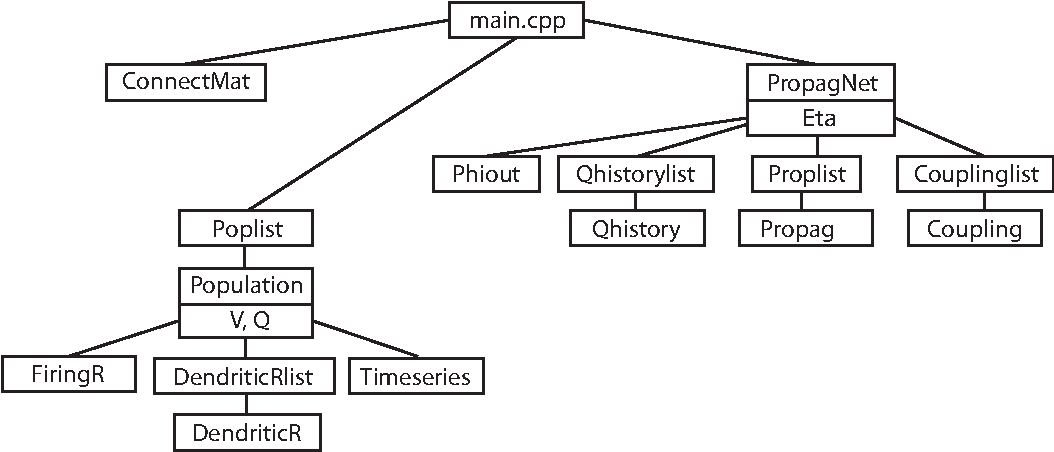
\includegraphics[scale=.8]{class.pdf}\caption{}\end{center}\end{figure}

\subsection{Class NF}
\label{sec:nf}

\textbf{ALL} classes that requires the configuration file should derive from the \type{NF} object. This abstract base class contains 3 member variables, and 5 interface methods:

\begin{tabular}{l p{10cm}}
Variable\\[6pt]
\type{nodes}&The number of nodes as specified from the configuration file.\\
\type{deltat}&The time increment per timestep in units of seconds.\\
\type{index}&The index associated with the object.\\[6pt]
Methods\\[6pt]
\type{init(Configf\& configf)}&Initializes the object with the config file.\\
 \type{dump(Dumpf\& dumpf) const}&When the program terminates, all objects dump information into a dump file (\type{dumpf}) for later restart. \type{Dumpf} is an \type{ofstream}.\\
\type{restart(Restartf\& restartf)}&Restarts the object in restart mode, \emph{in addition} to \type{init()}. The developer should have dumped all relevant information in dump, then reads it here.\\
\type{step(void)}&At each timestep, this function is called.\\
\type{output(Output\& output) const}&Specifies which fields to output.\\
\end{tabular}

All \type{NF} classes automatically handles the \type{ofstream::<<} and \type{ifstream::>>} operators.

\subsection{Class Array}
\label{sec:array}

\type{Array} is a container array to store objects that supports the \type{ofstream::<<} and \type{ifstream::>>} operators, as well as a \type{step(void)} function. This object typically is, but not necessarily has to be an \type{NF} object.

The \type{step(void)} function is equivalent to a \type{foreach(element).step()} in pseudocode. This function is encouraged over the use of \type{empty()}, \type{size()}, and \type{operator[]()}, which are discouraged to be used.

\subsection{Class Population}
\label{sec:newpop}

Models a neural population, which may be either a stimulus or normal population. If it has any dendrites, i.e. it has presynaptic connections, then it is a normal population, and it is a stimulus if it does not have dendrites.

In the former case, it contains the \type{QResponse} class and have a soma potential; in the latter case it contains the \type{Timeseries} class, and does not have a soma potential. See Fig.~\ref{fig:class} for reference.

In either cases, the \type{Population} class has a keyring storing the firing rate history, coded as a 2D array plus an integer key.

A population is ``settled" after \type{Population::init()} is called, after which no dendrites can be added, and the firing rate history cannot grow.

\subsection{Input/Output}

Input via the configuration file is implemented in the \type{init()} function, via \type{Configf}, which provides the following functions:
	\begin{enumerate}
	\item next: go to the next keyword
	\item param: go to the next keyword and reads in a variable. If the keyword is not found, barks and exits.
	\item optional: same as param, but does not bark nor exit.
	\item find: search a keyword and return the next variable as string.
	\end{enumerate}

In restart mode, \type{init()} is called, followed by \type{restart()}. \type{Restartf} is identical to \type{Configf}.

There are two modes of output. One is outputting the solution in \type{Population::output(), \type{Dendrite::output()}, \type{Propag::output()}}, and \type{Couple::output()}, and the other is the dumping of data for restart implemented in \type{dump()}.

To output field solutions, overload \type{NF::output()} to write
\begin{lstlisting}
output.prefix("Object Name",index+1);
output("field1",field1);
output("field2",field2);
output("field3",field3);
subobject1.output(output);
subobject2.output(output);
\end{lstlisting}
or for a single output field,
\begin{lstlisting}
output("Object Name",index+1,"field1",field1);
\end{lstlisting}

%To output solutions, return a vector of pointers to \type{new Output}, specifying the name and field of the solution. The name must be of the format
%\begin{lstlisting}
%label("Object.",index+1)+".field"
%\end{lstlisting}
%where \type{Object} and \type{field} should be appropriately named.

\type{dumpf()} provides a \type{Dumpf} object, which is essentially an \type{ofstream}. Dump all data here, so that it can be read in \type{restart()}.

\subsection{Writing a new class}

In extending \NF it is likely new classes needs to be written. When doing this, it would be useful to keep in mind:
\begin{enumerate}
	\item When appropriate, the default constructor, copy constructor, and \type{operator=} should be made inaccessible by declaring them to be private.
	\item If the configuration file is used, the \type{NF} class \textbf{MUST} be inherited.
	\item The \type{init()}, \type{restart()}, \type{dump()}, \type{step()} functions should be overloaded appropriately. Keep in mind that \type{restart()} internally calls \type{init()} at the beginning.
	\item \type{Population}, \type{Propag}, and \type{Couple} has the \type{output()} function to specify which field(s) to output. Overload this if appropriate.
	\item When in doubt, read existing class implementations for examples.
\end{enumerate}

\subsubsection{Class Propag}
\label{sec:newpropag}

The \type{Propag} class implements the axonal propagation as an identity map, i.e.
\[ \mathcal{D}_{ab} = 1. \]

To introduce more sophisticated axonal propagation, this class is inherited and overloaded.

The \type{Propag} class provides a constant references to both presynaptic and postsynaptic populations.

For finite differences integration, \type{Stencil} provides a 9-point stencil. To use, initialize it with a \type{vector<double>}, then access the Moore grid with \type{nw}, \type{n}, ... . Loop over the stencil with the operator \type{++}.

To ``register" your propagator, look for the
\begin{lstlisting}
// PUT YOUR PROPAGATORS HERE
\end{lstlisting}
section in \type{solver.cpp}.

\subsubsection{Class Couple}
\label{sec:newcouple}

The \type{Couple} class manages \(\nu_{ab}\), which is constant in space and time.

To introduce synaptic plasticity, derive from this class.

The \type{Couple} class provides a constant references to both presynaptic and postsynaptic populations. Glutamate concentration is also provided. \type{pos} is $+1$ or $-1$, depending on the sign of \(\nu_{ab}\).

To ``register" your couple, look for the
\begin{lstlisting}
// PUT YOUR COUPLES HERE
\end{lstlisting}
section in \type{solver.cpp}.

\subsubsection{Stimulus}

To implement new stimulus pattern, inherit from class \type{Timeseries}, where \type{init()} and \type{fire()} should be overloaded.

To ``register" your stimulus, look for the
\begin{lstlisting}
// PUT YOUR TIMEFUNCTION HERE
\end{lstlisting}
section in \type{timeseries.cpp}.

\subsection{Program flow}

Essentially, the program flow can be read from Fig.~\ref{fig:class}, so that objects take priority from top to bottom, left to right, both in terms of initialization and stepping through each timestep. A more detailed description is given below, and the reader is referred to the source code for complete description.

We use the semicolon to denote a succession of functions/procedures, and \type{a()} $\Rightarrow$ \type{b()} symbol to denote function \type{b()} as content of function \type{a()}.

\begin{center}
\begin{tabular}{ | l l p{11cm} | }
\hline \\

\type{main()}& $\Rightarrow$ &Initialize the config file, dump file and output file;\\[6pt]
&&\type{Solver::init()};\type{Solver::solve()};\\[6pt]
\type{Solver::init()}& $\Rightarrow$ &read in global parameters; Read in \type{CntMat};\\[6pt]
&&Construct \type{Population}; construct \type{Propag}; construct \type{Couple}; \type{Population::add2Dendrite()};\\[6pt]
&&Read configurations for \type{Population}, \type{Propag}, \type{Couple}, and \type{Output}.\\[6pt]
\type{Solver::solve()}& $\Rightarrow$ & \type{for(...) \{ Solver::step(); \type{Output::step()}; \} }\\[6pt]
\type{Solver::step()}& $\Rightarrow$ & \type{Population::step()}; \type{Propag::step()}; \type{Couple::step()};\\[6pt]
\type{Population::step()}& $\Rightarrow$ & \type{QResponse::step()} if neural population;\\[6pt]
&&\type{Timeseries::step()} if stimulus\\[6pt]
\type{QResponse::step()}& $\Rightarrow$ & \type{Dendrite::step()}; sum over \(V_{ab}\)

\\\hline
\end{tabular}
\end{center}

\begin{itemize}
\item One integration step of the model implements the following stages: 1) Dendritic response 2) Afferent summation. 3) Firing response/stimulus response. 4) Wave equation integration step which includes Q delay processing 5) Coupling response.
\item Most of the computational load comes from integrating wave equations and harmonic oscillators within the dendritic responses. Most computational time is probably on outputting.
\item Wave equations are integrated by explicit finite differences integration. A nine point spatial stencil is used to reduce high frequency spatial instabilities when driven by random noise. Other parts of code are unaffected by spatial geometry so this can be switched to irregular gridding easily.
\item Harmonic oscillators with dendritic rseponse are integrated using a heavily strength reduced explicit direct integration assuming constant drive. This was more efficient than a constant drive RK4 algorithm which would not be fourth order in any case due to the constant drive. Rennie used a constant drive RK4 for his 1997 code.
\end{itemize}

\subsection{Tools for solving differential equations}

Classes \type{DE} and \type{Integrator} (currently RK4 is implemented) are used to solve generic systems of ODEs, where the dynamical variables are homogeneous fields. For inhomogeneous DEs and spatial dependency, a 9-point stencil is provided in \type{Stencil}.

\begin{description}
	\item[DE] To solve ODEs of homogeneous fields, inherit \type{DE} and define the purely virtual \type{rhs()} function. Instantiate a \type{DE} object and an integrator, then step through it with \type{integrator.step()}. \type{STP} is an example using classes \type{DE} and \type{RK4}.
	\item[Stencil] Use \type{operator=} to apply a \type{Stencil} to a \type{vector<double>}, Then increment the stencil with \type{operator++}. The 9 stencil points can be read with \type{nw()} ... \type{se()}.
\end{description}

%\subsection{Other classes}

%\begin{description}
%\item[Modcouple] A class which provides synaptic coupling following a model proposed by Clearwater-Rennie for modelling neurotransmitter dynamics.
%\item[Random] Generates random numbers for Timeseries.
%\end{description}

\subsection{Submission to SVN}
The SVN repository is a standard installation, so any tutorials on usage of SVN apply here. For developers, we suggest obtaining a copy of the entire repository with

\begin{lstlisting}
svn co http://silliac.physics.usyd.edu.au:18080/svn/neurofield/ neurofield --username=<your SVN username>
\end{lstlisting}
	
The following folders are present:

\begin{tabular}{l p{12cm}}
\type{branches}& Folders for users to make changes to the program.\\
\type{tags}& Previous versions of the program.\\
\type{trunk}& Latest stable version of the program.\\
\end{tabular}

To make changes to the program, it is recommended to copy the trunk into a new subfolder within branches

\begin{lstlisting}
cp -r trunk ./branches/my_branch
\end{lstlisting}
	
You can then freely modify the code in the branch with the benefit of version control, and other users can obtain your code through the branch. If your modifications are accepted for the main program, your branch will then be merged into the trunk subject to appropriate testing.

\subsection{TODO}
\begin{enumerate}
\item check numerical entry of connection matrix
\item restart mode has never been used. Leave it that way.
\end{enumerate}
\end{document}
